%
% ---------------------------------------------------
%
% Trabajo Fin de Grado:
% Author: Laura Padrón Jorge <gonzalezsuarezivan@gmail.com>
% Author: F. de Sande fsande@ull.es
% Fichero: main.tex
%
% ----------------------------------------------------
%
\documentclass[spanish,a4paper,14pt,oneside]{extreport}
%\documentclass[a4paper, twoside, 12pt]{book}
\usepackage[a4paper]{geometry}
\usepackage[spanish]{babel}
\usepackage[utf8]{inputenc}
%\usepackage{lscape}
\usepackage{pdflscape}
%%%%%%%%%%%%%%%%%%%%%%%%%%%%%%%%%%%%%%%%%%%%%%%%%%%%%%%%%%%%%%%%%%%%%%%%%%%%%%%%%%%%%%%%%%%%
% Next 3+3 lines select PDF or PS output (comment as apropriate)
% To switch from PDF and PS comment/uncomment here and change Makefile
\usepackage[pdftex]{color}
\usepackage[pdftex]{graphicx}
\graphicspath{{images/}}
%\usepackage[dvips]{color}
%\usepackage[dvips]{graphicx}
\usepackage{epsfig}
%\graphicspath{{images/eps/}} 
%%%%%%%%%%%%%%%%%%%%%%%%%%%%%%%%%%%%%%%%%%%%%%%%%%%%%%%%%%%%%%%%%%%%%%%%%%%%%%%%%%%%%%%%%%%%
\usepackage{algorithmic}
\usepackage[pdftex=true,colorlinks=false,urlcolor=blue,plainpages=false,pagebackref=true,citecolor=red]{hyperref} %hiperenlaces y backcites 
%%%%%%%%%%%%%%%%%%%%%%%%%%%%%%%%%%%%%%%%%%%%%%%%%%%%%%%%%%%%%%%%%%%%%%%%%%%%%%%%%%%%%%%%%%%%
% Comandos para escribir "siempre igual"
\newcommand{\BulletPoint}{\texttt{BulletPoint{}}}

%%% Traducimos el pseudocodigo
\renewcommand{\algorithmicwhile}{\textbf{mientras}}
\renewcommand{\algorithmicend}{\textbf{fin}}
\renewcommand{\algorithmicdo}{\textbf{hacer}}
\renewcommand{\algorithmicif}{\textbf{si}}
\renewcommand{\algorithmicthen}{\textbf{entonces}}
\renewcommand{\algorithmicrepeat}{\textbf{repetir}}
\renewcommand{\algorithmicuntil}{\textbf{hasta que}}
\renewcommand{\algorithmicelse}{\textbf{en otro caso}}
\renewcommand{\algorithmicfor}{\textbf{para}}

%%%%%%%%%%%%%%%%% Creamos un entorno para listar código fuente %%%%%%%%%%%%%%%
\newenvironment{sourcecode}
{\begin{list}{}{\setlength{\leftmargin}{1em}}\item\scriptsize\bfseries}
{\end{list}}

\newenvironment{littlesourcecode}
{\begin{list}{}{\setlength{\leftmargin}{1em}}\item\tiny\bfseries}
{\end{list}}

\newenvironment{summary}
{\par\noindent\begin{center}\textbf{Abstract}\end{center}\begin{itshape}\par\noindent}
{\end{itshape}}

\newenvironment{keywords}
{\begin{list}{}{\setlength{\leftmargin}{1em}}\item[\hskip\labelsep \bfseries Keywords:]}
{\end{list}}

\newenvironment{palabrasClave}
{\begin{list}{}{\setlength{\leftmargin}{1em}}\item[\hskip\labelsep \bfseries Palabras clave:]}
{\end{list}}


%%%%%%%%%%%%%%%%%%%%%%%%%%%%%%%%%%%%%%%%%%%%%%%%%%%%%%%%%%%%%%%%%%%%%%%%%%%%%%%
\definecolor{marron}       {rgb}{0.496, 0.203, 0.152}
\definecolor{verde-claro}  {rgb}{0.625, 0.734, 0.199}
\definecolor{oscuro}       {rgb}{0.187, 0.141, 0.285}
\definecolor{gris}     	   {rgb}{0.500, 0.500, 0.500}
\definecolor{bgd-listings} {rgb}{0.999, 0.999, 0.900}
\definecolor{gray97}{gray}{.97}
\definecolor{gray75}{gray}{.75}
\definecolor{gray45}{gray}{.45}
\definecolor{gray}{gray}{.45}
%%%%%%%%%%%%%%%%%%%%%%%%%%%%%%%%%%%%%%%%%%%%%%%%%%%%%%%%%%%%%%%%%%%%%%%%%%%%%%%%%%%%%%%%%%%%
%%% Code Listings
%\usepackage{listings} 
%\lstloadlanguages{python,C}
\definecolor{Brown}{cmyk}{0,0.81,1,0.60}
\definecolor{OliveGreen}{cmyk}{0.64,0,0.95,0.40}
\definecolor{CadetBlue}{cmyk}{0.62,0.57,0.23,0}
\definecolor{lightlightgray}{gray}{0.9}
%%%%%%%%%%%%%%%%%%%%%%%%%%%%%%%%%%%%%%%%%%%%%%%%%%%%%%%%%%%%%%%%%%%%%%%%%%%%%%%%%%%%%%%%%%%
%Evitar partir palabras al final de la línea
%\hyphenpenalty=10000
%\tolerance=1000
%%%%%%%%%%%%%%%%%%%%%%%%%%%%%%%%%%%%%%%%%%%%%%%%%%%%%%%%%%%%%%%%%%%%%%%%%%%%%%%%%%%%%%%%%%%%
% Para listados de código
\usepackage{listings}
\lstloadlanguages{C}

% Definiendo colores para los listados de código fuente - Univ. Deusto
\definecolor{violet}{rgb}{0.5,0,0.5}
\definecolor{navy}{rgb}{0,0,0.5}
\definecolor{hellgelb}{rgb}{1,1,0.8}
\definecolor{colKeys}{rgb}{0,0,1}
\definecolor{colIdentifier}{rgb}{0,0,0}
\definecolor{colComments}{rgb}{1,0,0}
\definecolor{colString}{rgb}{0,0.5,0}

%\lstset{morekeywords={pragma copy\_in copy\_out copy omp parallel private reduction shared hicuda loop\_partition over\_tblock over\_thread}}
\lstset{
        float=tbhp,
		    language = Java,
				morekeywords={llc,reduction_type,nc_result,
				              hicuda,global,alloc,shape,kernel,thread,loop_partition,tblock,over_tblock,over_thread,kernel_end,copyout,free,
											data,region,
											task,input,inout,output,
				              pragma,omp,parallel,reduction,private,shared,target,device,copy_in,copy_out,
				              acc,kernels,loop,copyin,copy,pcopy,pcopyin,collapse,gang,worker,independent},
				%\emph      ={omp,parallel,reduction,private,shared},
				emphstyle=\textbf,
        %basicstyle=\ttfamily\tiny,
        basicstyle=\ttfamily\scriptsize,
        identifierstyle=\color{colIdentifier},
        keywordstyle=\color{colKeys},
        stringstyle=\color{colString},
        commentstyle=\color[rgb]{0.133,0.545,0.133},
        columns=flexible,
        tabsize=4,
        frame=single,
        extendedchars=true,
        showspaces=false,
        showstringspaces=false,
        numbers=left,
        numberstyle=\tiny,
        breaklines=true,
        backgroundcolor=\color{lightlightgray},
        breakautoindent=true,
        captionpos=b
}

%\renewcommand{\lstlistingname}{Listing} % Los títulos de los códigos insertados se denotan con Ejemplo...   

% Otro formato más bonito para código fuente
\newcommand{\codigofuente}[3]{%
  \lstlisting[language=#1,caption={#2}]{#3}%
}
%%%%%%%%%%%%%%%%%%%%%%%%%%%%%%%%%%%%%%%%%%%%%%%%%%%%%%%%%%%%%%%%%%%%%%%%%%%%%%%
\begin{document}
\renewcommand{\lstlistingname}{Listado}% Listing -> Listado de código
%%%%%%%%%%%%%%%%%%%%%%%%%%%%%%%%%%%%%%%%%%%%%%%%%%%%%%%%%%%%%%%%%%%%%%%%%%%%%%%
% First Page
%%%%%%%%%%%%%%%%%%%%%%%%%%%%%%%%%%%%%%%%%%%%%%%%%%%%%%%%%%%%%%%%%%%%%%%%%%%%%%%

\pagestyle{empty}
\thispagestyle{empty}


\newcommand{\HRule}{\rule{\linewidth}{1mm}}
\setlength{\parindent}{0mm}
\setlength{\parskip}{0mm}

\vspace*{\stretch{0.5}}

\begin{center}

\includegraphics[scale=0.8]{images/logo_vertical}\\[10mm]
{\Huge Trabajo de Fin de Grado}
\end{center}

\HRule
\begin{flushright}
        {\Huge \BulletPoint{}} \\[2.5mm]
        {\Large Laura Padrón Jorge} \\[5mm]


\end{flushright}
\HRule
\vspace*{\stretch{2}}
\begin{center}
  \Large La Laguna, \today
\end{center}

\setlength{\parindent}{5mm}

%%%%%%%%%%%%%%%%%%%%%%%%%%%%%%%%%%%%%%%%%%%%%%%%%%%%%%%%%%%%%%%%%%%%%%%%%%%%%%%
% Signature page (add the official stamp)
%%%%%%%%%%%%%%%%%%%%%%%%%%%%%%%%%%%%%%%%%%%%%%%%%%%%%%%%%%%%%%%%%%%%%%%%%%%%%%%
\newpage
%\cleardoublepage
\thispagestyle{empty}

D. {\bf Francisco de Sande González}, con N.I.F. 42.067.050-G
profesor
Titular de Universidad
adscrito al Departamento
de Ingeniería Informática y de Sistemas
de la Universidad de La Laguna, como tutor

\bigskip

\bigskip
\bigskip
{\bf C E R T I F I C A}

\bigskip
\bigskip
\bigskip
Que la presente memoria titulada:

\bigskip
``{\it \BulletPoint{}}''

\bigskip
\bigskip
\bigskip
%Cambiar
\noindent ha sido realizada bajo su dirección por Dñ. {\bf Laura Padron Jorge},
con N.I.F. 79.890.251-W

\bigskip
\bigskip

Y para que así conste, en cumplimiento de la legislación vigente y a los efectos
oportunos firman la presente en La Laguna a \today

%\cleardoublepage
\newpage
%%%%%%%%%%%%%%%%%%%%%%%%%%%%%%%%%%%%%%%%%%%%%%%%%%%%%%%%%%%%%%%%%%%%%%%%%%%%%%%
\thispagestyle{empty}

{ \flushright

\begin{LARGE}
Agradecimientos
\end{LARGE}

\hspace{3mm}

\begin{large}


\hspace{3mm}
%Agradecimientos


\end{large}

}

%%%%%%%%%%%%%%%%%%%%%%%%%%%%%%%%%%%%%%%%%%%%%%%%%%%%%%%%%%%%%%%%%%%%%%%%%%%%%%%%%
\newpage

\begin{huge}
Licencia
\end{huge}

\bigskip
%* Si quiere permitir que se compartan las adaptaciones de tu obra mientras se comparta de la misma manera
%y NO quieres permitir usos comerciales de tu obra indica:

\begin{center}

\includegraphics[scale=1.5]{images/by-nc-sa_88x31}\\[10mm]
{\Large \copyright~Esta obra está bajo una licencia de Creative Commons Reconocimiento-NoComercial-CompartirIgual 4.0 Internacional.
}
\end{center}


%%%%%%%%%%%%%%%%%%%%%%%%%%%%%%%%%%%%%%%%%%%%%%%%%%%%%%%%%%%%%%%%%%%%%%%%%%%%%%%
\newpage  %\cleardoublepage
\begin{abstract}
{\em

El objetivo de este trabajo ha sido el desarrollo de una aplicación para dispositivos Android, que además utilice una de las tecnologías más recientesen el mercado actual, los Beacons.

\bigskip
Partiendo de los conocimientos en \textit{Java} obtenidos en la asignatura: \textit{'Diseño arquitectónico y patrones'} cursada en el 
itinerario de Ingeniería del Software, (impartida en el tercer curso del Grado en Ingeniería Informática de la Universidad de La Laguna), se espera adquirir los conocimientos necesarios para desarrollar aplicaciones en Android.

\bigskip
Asimismo, se espera dotar al alumno de independencia en su trabajo, visión y planificación. Desarrollo de tareas de investigación, documentación, desarrollo y despliegue utilizando tanto los conocimientos adquiridos durante la carrera, como aquellos que se irán aprendiendo durante el progreso de trabajo.

\bigskip 
También se espera adquirir soltura y familiarizarse con el uso de los "Beacons". Se espera que el alumno investigue y aprenda de una tecnología reciente, que si bien aún no tiene un impacto muy grande en el mercado, en unos años se espera que se empiece a utilizar con naturalidad en distintos ámbitos, Turismo, Enseñanza o en el ámbito Comercial.

}
\begin{palabrasClave}
Aplicaciones Android, Beacons.
\end{palabrasClave}

\end{abstract}
%%%%%%%%%%%%%%%%%%%%%%%%%%%%%%%%%%%%%%%%%%%%%%%%%%%%%%%%%%%%%%%%%%%%%%%%%%%%%%%

%%%%%%%%%%%%%%%%%%%%%%%%%%%%%%%%%%%%%%%%%%%%%%%%%%%%%%%%%%%%%%%%%%%%%%%%%%%%%%%
\newpage  %\cleardoublepage
\begin{summary}
{\em

The aim of the Project has been the development of an application for Android devices which will be using beacon technology for some of main its main features.

\bigskip
Based on the knowledge of Java obtained in the subject: ''Architectural Design and Patterns'' taken in the
Software Engineering Branch (Given in third year of Computing Engineering Degree from ''La Universidad de La Laguna''). 
in this work we expect to acquire the basic knowledge needed to
develop Android applications introducing us in the development of applications related to Beacon Technology.

\bigskip
Moreover, it is expected for the student to learn independency in her work and to gain vision and planification aptitudes when working on a project. Developing differents labours of investigation, documentation, development and deployment using the knowledge adquired during the Degree and within the development of this project.

\bigskip
Apart from all this, it's of great importance to get to know this new Beacon technolgy. We want the student to investigate and learn by herselft a recent technology, which if not at the moment is well know, in the next future it is expected to get more attention in differents sectors, such as Tourism, Learning or Trading.
}

\begin{keywords}
Application for Android, Beacons.
\end{keywords}

\end{summary}
%%%%%%%%%%%%%%%%%%%%%%%%%%%%%%%%%%%%%%%%%%%%%%%%%%%%%%%%%%%%%%%%%%%%%%%%%%%%%%%

%%%%%%%%%%%%%%%%%%%%%%%%%%%%%%%%%%%%%%%%%%%%%%%%%%%%%%%%%%%%%%%%%%%%%%%%%%%%%%%
\newpage{\pagestyle{empty}}
\thispagestyle{empty}

%%%%%%%%%%%%%%%%%%%%%%%%%%%%%%%%%%%%%%%%%%%%%%%%%%%%%%%%%%%%%%%%%%%%%%%%%%%%%%%


\pagestyle{myheadings} %my head defined by markboth or markright
% No funciona bien \markboth sin "twoside" en \documentclass, pero al
% ponerlo se dan un montón de errores de underfull \vbox, con lo que no se
% ha puesto.
\markboth{Laura Padrón Jorge}{BulletPoint}

%%%%%%%%%%%%%%%%%%%%%%%%%%%%%%%%%%%%%%%%%%%%%%%%%%%%%%%%%%%%%%%%%%%%%%%%%%%%%%%
%Numeracion en romanos
\renewcommand{\thepage}{\roman{page}}
\setcounter{page}{1}

%%%%%%%%%%%%%%%%%%%%%%%%%%%%%%%%%%%%%%%%%%%%%%%%%%%%%%%%%%%%%%%%%%%%%%%%%%%%%%%

\tableofcontents

%%%%%%%%%%%%%%%%%%%%%%%%%%%%%%%%%%%%%%%%%%%%%%%%%%%%%%%%%%%%%%%%%%%%%%%%%%%%%%%
\newpage{\pagestyle{empty}}

\listoffigures

%%%%%%%%%%%%%%%%%%%%%%%%%%%%%%%%%%%%%%%%%%%%%%%%%%%%%%%%%%%%%%%%%%%%%%%%%%%%%%%
\newpage{\pagestyle{empty}}

%\listoftables

%%%%%%%%%%%%%%%%%%%%%%%%%%%%%%%%%%%%%%%%%%%%%%%%%%%%%%%%%%%%%%%%%%%%%%%%%%%%%%%
\newpage{\pagestyle{empty}}

%%%%%%%%%%%%%%%%%%%%%%%%%%%%%%%%%%%%%%%%%%%%%%%%%%%%%%%%%%%%%%%%%%%%%%%%%%%%%%%
%Numeracion a partir del capitulo I
\renewcommand{\thepage}{\arabic{page}}
\setcounter{page}{1}


%%%%%%%%%%%%%%%%%%%%%%%%%%%%%%%%%%%%%%%%%%%%%%%%%%%%%%%%%%%%%%%%%%%%%%%%%%%%%%%
%\chapter{Introducción}
%\label{chapter:intro}
%\input{cap1.tex}
%%%%%%%%%%%%%%%%%%%%%%%%%%%%%%%%%%%%%%%%%%%%%%%%%%%%%%%%%%%%%%%%%%%%%%%%%%%%%%%
%\chapter{Título del Capítulo Dos}
%\label{chapter:dos}
%\input{cap2.tex}
%%%%%%%%%%%%%%%%%%%%%%%%%%%%%%%%%%%%%%%%%%%%%%%%%%%%%%%%%%%%%%%%%%%%%%%%%%%%%%%%
%\newpage{\pagestyle{empty}}
%\thispagestyle{empty}
%\chapter{Título del Capítulo Tres}
%\label{chapter:tres}
%\input{cap3.tex}
%%%%%%%%%%%%%%%%%%%%%%%%%%%%%%%%%%%%%%%%%%%%%%%%%%%%%%%%%%%%%%%%%%%%%%%%%%%%%%%%
%\chapter{Título del Capítulo Cuatro}
%\label{chapter:cuatro}
%\input{cap4.tex}
%%%%%%%%%%%%%%%%%%%%%%%%%%%%%%%%%%%%%%%%%%%%%%%%%%%%%%%%%%%%%%%%%%%%%%%%%%%%%%%%
%\newpage{\pagestyle{empty}}
%\thispagestyle{empty}
%\chapter{Conclusiones y líneas futuras}
%\label{chapter:Conclusiones}
%\input{cap5.tex}
%%%%%%%%%%%%%%%%%%%%%%%%%%%%%%%%%%%%%%%%%%%%%%%%%%%%%%%%%%%%%%%%%%%%%%%%%%%%%%%%
%\newpage{\pagestyle{empty}}
%\thispagestyle{empty}
%\chapter{Summary and Conclusions }
%\label{chapter:ingles}
%\input{cap6.tex}
% ==========================================================
% --------               Capítulos                ----------
% --------    Estan en el directorio capitulos/   ----------
% ==========================================================
% ---------------------------------------------------
%
% Proyecto de Final de Carrera: 
% Author: Laura Padron Jorge <alu0100703511@ul.edu.es>
% Introducción
% Fichero: Prologo.tex
%
% ----------------------------------------------------

\chapter*{Introducción}
\addcontentsline{toc}{chapter}{Introducción} 

Este documento comprende el trabajo de investigación y desarrollo realizado por la alumna en la consecución de su Trabajo de Fin de Grado (TFG), con el que culminará sus estudios del Grado en Ingeniería Informática cursados en la Escuela Superior de Ingeniería y Tecnología (ESIT) de la Universidad de la Laguna (ULL).

%
% ---------------------------------------------------
%
% Proyecto de Final de Carrera:
% Author: Laura Padrón Jorge <alu0100703511@ull.edu.es>
% Capítulo: Objetivos 
% Fichero: Cap1_Goals.tex
%
% ----------------------------------------------------
%


\chapter{Objetivos} \label{chap:Objetivos}  

Este TFG tiene los siguientes objetivos principales:

	
\begin{itemize}
\item  	Por un lado se pretende ampliar los conocimientos en tecnologías móviles en el sistema operativo \textit{Android} \cite{URL::Android} y en el desarrollo de aplicaciones para este sistema operativo.
\item Por otro lado, también se pretende que la alumna se familiarice con el uso de herramientas de control de versiones utilizando GitHub \textit{Github} \cite{URL::Github} y de edición de textos técnicos utilizando \textit{LaTeX}  \cite{URL::LaTeX}.
\item Otro objetivo presente en este TFG es que la alumna investigue y profundice en una tecnología reciente en el mercado, los \textit{Beacons} \cite{URL::Beacon}.
\item  Por último, se espera que la estudiante obtenga independencia en su trabajo, visión y planificación poniendo en marcha tareas de investigación, documentación, desarrollo y despliegue utilizando tanto los conocimientos adquiridos durante la carrera, como aquellos que se irán aprendiendo durante el progreso de este trabajo.
\end{itemize}
%% ---------------------------------------------------
%
% Proyecto de Final de Carrera:
% Author: Laura Padrón Jorge <alu0100703511@ull.edu.es>
% Capítulo: Herramientas de Desarrollo utilizadas 
% Fichero: Cap2_SoftwareTools.tex
%
% ----------------------------------------------------
%


\chapter{Herramientas de Desarrollo utilizadas} \label{chap:HerramientasSoftware}

Este capitulo tiene como objetivo presentar las distintas Herramientas Software empleadas por la alumna en el desarrollo de su TFG.

\section{Android Studio}

Android Studio \cite{URL::AndroidStudio} es el IDE(Entorno de Desarrollo Integrado) oficial para el desarrollo de aplicaciones en Android, basado en IntelliJ IDEA \cite{URL::IntelliJIDEA}. Android Studio ofrece una serie de funcionalidades que han facilitado a la desarrolladora numerosas tareas, entre ellas podemos destacar:


\begin{itemize}
\item Un sistema de compilación basado en Gradle que ha facilitado la inserción de dependencias de las distintas librerías que se han tenido que utilizar.
\item Un emulador rápido y fácil de utilizar, que en este caso no ha sido de mucha ayuda para probar el funcionamiento, ya que dependía de la tecnología Bluetooth, pero ha ayudado a visualizar las distintas pantallas en algunos momentos.
\item La facilidad para publicar cambios a aplicaciones ya funcionando sin tener que compilar un nuevo APK.
\item Plantillas de código e integración con GitHub para utilizar funcionalidades comúnes en la mayoría de las aplicaciones.
\item Un sistema de visualización de las diferentes pantallas muy completo, con soporte visual para añadir componentes y cambiar atributos fácilmente.
\item Un sistema de depuración, con una interfaz sencilla y completa.
\end{itemize} 

\begin{figure}[h]
	\centering
	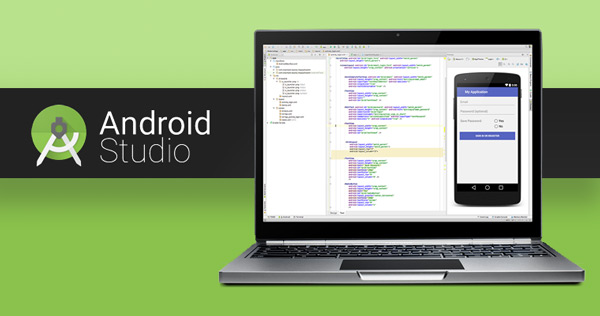
\includegraphics[width=\columnwidth]{androidstudio}
	\caption{Android studio, un IDE flexible e intuitivo.}
	\label{fig:androidstudio}
\end{figure}

Se ha utilizado este IDE frente a otros como Eclipse + ADT \cite{URL::eclipseADT} debido a que en la actualidad es el IDE oficial con soporte de Google. Se ha preferido aprender a utilizar este entorno con vistas al futuro, ya que en un futuro parece que se consolidará como el preferido para los desarrolladores Android.

\section{LaTex}

LaTeX \cite{URL::LaTeX} es un sistema de composición de textos, orientado a la creación de documentos escritos que presenten una alta calidad tipográfica. Por sus características y posibilidades, es usado de forma especialmente intensa en la generación de artículos y libros científicos que incluyen, entre otros elementos, expresiones matemáticas.


LaTeX está formado por un gran conjunto de macros de TeX, escrito por Leslie Lamport en 1984, con la intención de facilitar el uso del lenguaje de composición tipográfica, creado por Donald Knuth. Es muy utilizado para la composición de artículos académicos, tesis y libros técnicos, dado que la calidad tipográfica de los documentos realizados con LaTeX es comparable a la de una editorial científica de primera línea. LaTeX es software libre bajo licencia LPPL.


Se ha decidido utilizar este sistema debido al carácter profesional que le aporta a los documentos. Ha sido una buena oportunidad para aprender a utilizar un sistema de composición de texto como este, ya que en un futuro puede ser beneficioso el saber manejar esta herramienta. Si bien es cierto, que el uso de esta herramienta frente a otros editores más familiares ha sido algo tedioso en el inicio, es verdad que una vez acostumbrada a utilizarla ha resultado ser múy eficaz. A la hora de aprender a utilizar la herramienta, se han utilizado principalmente manuales por internet, alguno a destacar que se encuentra en español sería por ejemplo: \cite{URL::manualLatex}

\section{Github}

GitHub es una forja (plataforma de desarrollo colaborativo) para alojar proyectos utilizando el sistema de control de versiones Git. Utiliza el framework Ruby on Rails por GitHub, Inc. (anteriormente conocida como Logical Awesome). Desde enero de 2010, GitHub opera bajo el nombre de GitHub, Inc. El código se almacena de forma pública, aunque también se puede hacer de forma privada, creando una cuenta de pago.


Se ha decidido crear un repositorio en esta plataforma para poder llevar un control y una trazabilidad del proyecto. El tutor y la alumna han trabajado en este repositorio. En el caso del tutor, principalmente para revisar el seguimiento semanal y llevar un control de las tareas. Aparte de este repositorio, también se ha abierto un segundo asociado a la OSL para subir el código una vez terminado como parte del PFLT. Accesible libremente desde: \cite{URL::repositorioAplicacion}


Mediante el uso de este repositorio la alumna ha conseguido ampliar sus conocimientos en Git, y familiarizarse con la interfaz de GitHub. Previamente se había utilizado como repositorios GitLab, SVN y RTC en otros proyectos, por lo que no ha sido una complicación mayor utilizar este sistema.


\begin{figure}[h]
	\centering
	
\includegraphics[width=\columnwidth]{github}
	\caption{La plataforma de desarrollo colaborativo GitHub.}
	\label{fig:github}
\end{figure}
% ---------------------------------------------------
%
% Trabajo de Fin de Grado. 
% Author: Laura Padrón Jorge. 
% Capítulo: Tecnologías utilizadas en el Trabajo de Fin de Grado. 
% Fichero: Cap3_Technology.tex
%
% ----------------------------------------------------
%

\cleardoublepage
\chapter{Tecnologías} \label{chap:Tecnologias} 

En este capítulo se habla de las principales tecnologías que han sido utilizadas durante la elaboración de este TFG.


\section{El Sistema Operativo Android}

Con frecuencia anteriormente en el desarrollo de este documento hemos nombrado el Sistema Operativo (S.O) Android, pero ¿Qué es Android?

Android es un sistema operativo que emplea Linux en la interfaz del hardware.  Los componentes del SO subyacentes se escriben en C o C++ pero las aplicaciones diseñadas se escriben en Java. De esta manera Android asegura una amplia operatividad en una gran variedad de dispositivos debido a dos hechos: la interfaz en Linux ofrece gran potencia y funcionalidad para aprovechar el hardware de los futuros dispositivos, mientras que el hecho de que las aplicaciones se desarrollen en Java permite que Android sea accesible para un gran número de programadores conocedores del código.

Fue diseñado principalmente para dispositivos móviles con pantalla táctil, smartphones, tablets y otros dispositivos como televisores o automóviles. Inicialmente fue desarrollado por Android Inc., empresa que fue respaldada económicamente por Google y más tarde fue comprada por esta misma empresa.

Tiene una gran comunidad de desarrolladores creando aplicaciones para extender la funcionalidad de los dispositivos. A la fecha existen más de 1.000.000 de aplicaiones disponibles para la tienda de aplicaciones oficial de Android: Google Play \cite{URL::GooglePlay} sin tener en cuenta las aplicaciones de otras tiendas no oficiales para Android como la tienda de aplicaciones de Samsung Apps \cite{URL::SamsungApps}, Slideme…

\section{Los llamados Beacons}

Los \textit{''Beacons''} \cite{URL::Beacon}, cuya traducción del inglés equivaldría a \textit{''balizas''} o \textit{''faros''}, es una tecnología emergente que desde algunos años se está intentando abrir paso en el mercado. Como su propio nombre indica, estos dispositivos intentan dar una mejor solución al posicionamiento en interiores, siendo un mecanismo de guía en lugares donde otras tecnologías, como el GPS o el Wifi dejan de funcionar o resultan imprecisas. 

Sin embargo, estos no son los únicos usos de los beacons, actualmente muchas empresas están ampliando sus usos a otros campos, y el diseño de estos beacons se está presentando en tamaños tan pequeños y con un tiempo de funcionamiento tan elevado, que se pueden desplegar prácticamente en cualquier lugar sin dificultades.

A continuación se intentará responder a las preguntas más frecuentes que nos pueden surgir con respecto a esta tecnología:


\begin{itemize}
\item ¿Qué es un Beacon?
\item ¿Cómo funcionan estos dispositivos?
\item ¿Qué rango de alcance poseen?
\item ¿Con qué dispositivos móviles son compatibles? 
\item ¿Qué ventajas y desventajas tienen con respecto a otras tecnologías?
\item ¿Qué usos se le ha dado a esta tecnología hasta ahora?
\item ¿Qué empresas trabajan con esta tecnología?
\end{itemize}

\begin{figure}[!h]
        \begin{floatrow}
        \ffigbox{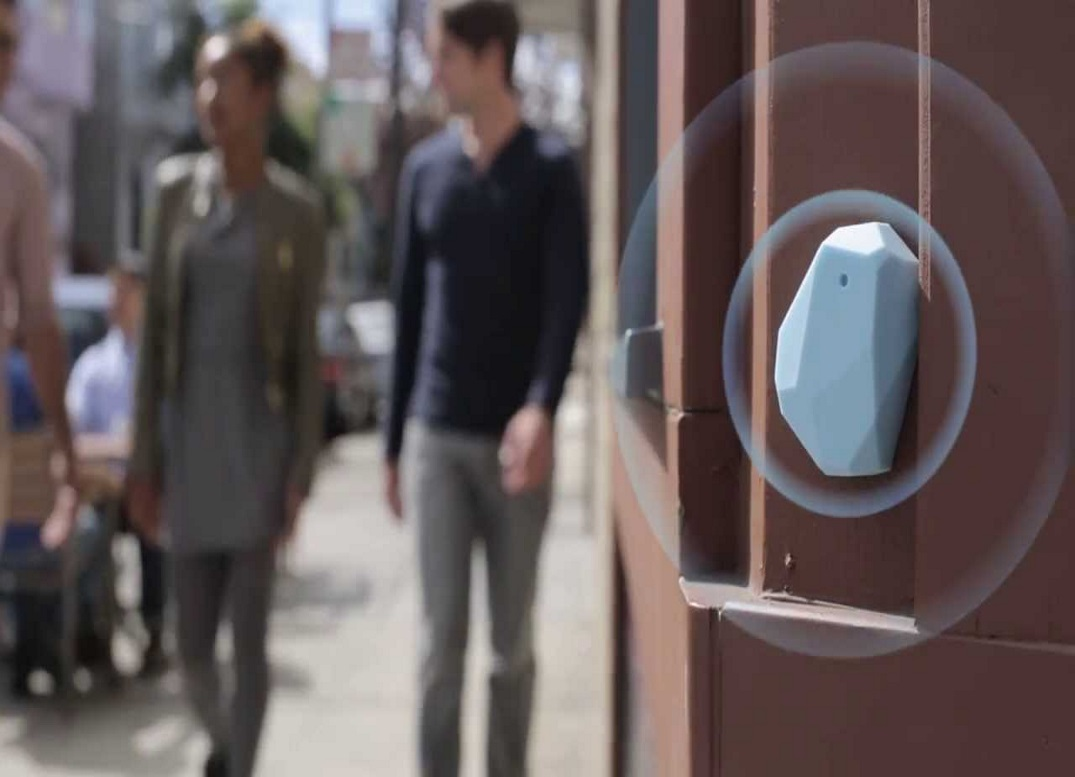
\includegraphics[width=\textwidth/2]{estimoteBeacon}}{\caption{Uno de los beacons de la compañia Estimote}\label{fig:estimote_Beacon}}
        \ffigbox{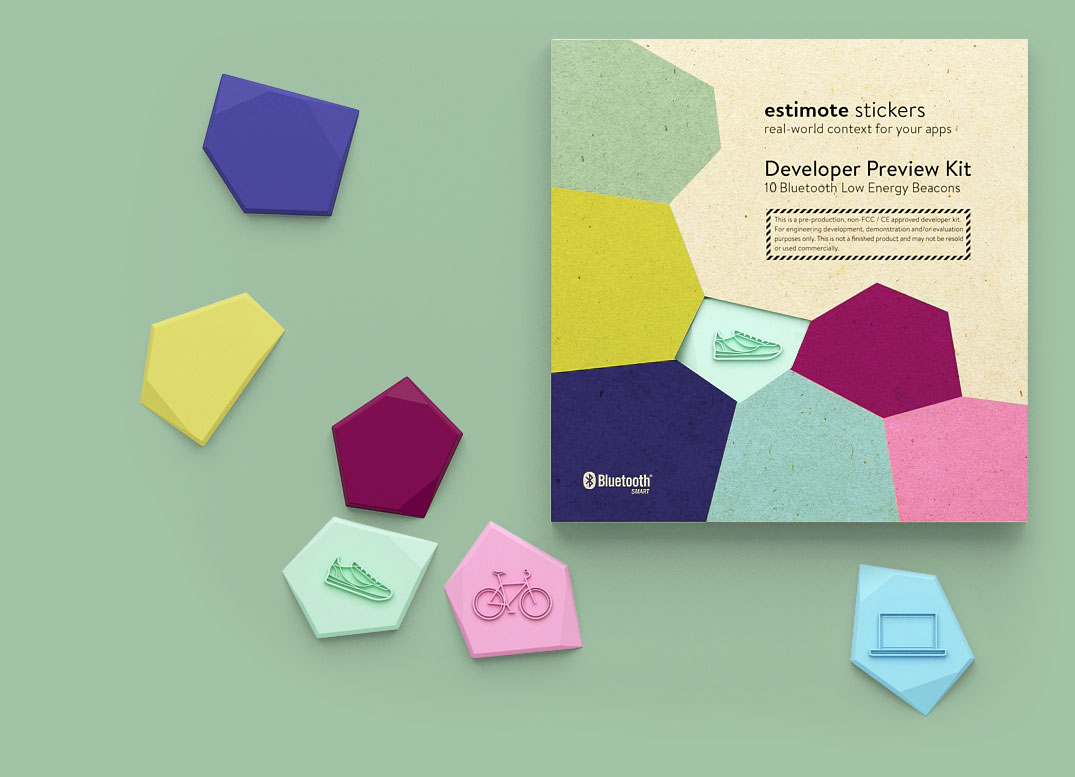
\includegraphics[width=\textwidth/2]{estimoteSticker}}{\caption{Uno de los beacons de la compañia Estimote en formato Pegatina}\label{fig:estimote_Beacon_Sticker}}
        \end{floatrow}
\end{figure}

\subsection{¿Qué es un Beacon?}

Para los que no hayan oido este término, en el marco en el que nos movemos, hace referencia a un pequeño dispositivo (sus tamaños varían de uno a otro, pero siempre de tamaño reducido) que emite señales de onda corta utilizando la tecnología Bluetooth \cite{URL::Bluetooth}. Estas señales contienen una pequeña cantidad de información y son recibidas por dispositivos móviles con tecnología Bluetooth dentro de un rango de cobertura variable dependiendo del propio dipositivo. Normalmente, la fuerza de esta señal y su frecuencia son configurables.

\begin{figure}[h]
	\centering
	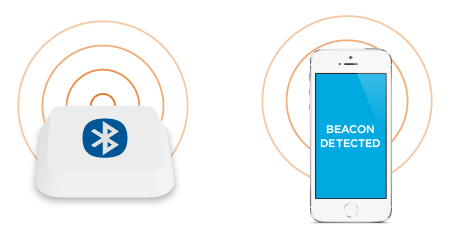
\includegraphics[width=\columnwidth]{beaconPhone}
	\caption{Representación de un beacon emitiendo mediante Bluetooth a un dispositivo móvil}
	\label{fig:beaconBluetooth}
\end{figure}

El funcionamiento de un beacon es sencillo: El beacon emite una señal ininterrumpida que es captada por los dispositivos móviles dentro de su radio de cobertura, esta señal contiene información capaz de definir una localización, detectar y localizar otros dispositivos. A continuación la señal es captada por una aplicación movil previamente instalada, que dependiendo de la señal recibida, puede lanzar una acción en dicho dispositivo.


Hay que tener en cuenta que esta señal es unilateral: los beacons son capaces de enviar señales pero no están preparados para recibirlas. También hay que tener en cuenta, que la mayoría de las beacon actuales en el mercado transmiten información preconfigurada, confiando en la aplicacion móvil para utilizar la información; sin embargo es muy posible que esto cambie en un futuro, ampliando las posibilidades de los beacons.

\subsection{¿Como funcionan estos dispositivos?}

Los beacons usan Bluetooth Low Energy (BLE) \cite{URL::BluetoothLowEnergy}, una version del protocolo Bluetooth diseñada para usar mucha menos energía y enviar menos información. Los beacons funcionan con baterías cuyo tiempo de vida depende de la configuración establecida, teniendo en cuenta la emisión de la señal (fuerza y frencuencia) y tiempo de hibernación. Sus tiempos de vida son variables, pudiendo durar desde un mes hasta varios años. 

\begin{figure}[h]
	\centering
	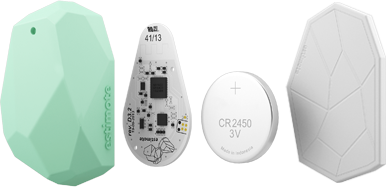
\includegraphics[width=\columnwidth]{estimoteBeaconInside}
	\caption{Interior de un beacon de Estimote}
	\label{fig:beaconInside}
\end{figure}

Independientemente de lo que se pueda pensar, los beacons en si mismas no transmiten información significativa, transmiten identificadores cortos junto con información customizable breve, que son interpretadas por una aplicación que sabe lo que tiene que hacer con esa información y que es la que se encarga de procesar la información y realizar una acción pertinente.

Este identificador se divide en tres partes: 

\begin{itemize}
\item \textit{''UUID''} \cite{URL::UUID} : corresponde con una ID dada por el vendedor e identifica el beacon en cuestión.
\item ID Superior : customizables y utilizadas con un significado específico que puede identificar una acción o parámetro. 
\item ID Inferior: customizables y utilizadas al igual que la superior con un significado específico que se puede usar para identificar una acción o parámetro.
\end{itemize}

\begin{figure}[h]
	\centering
	
\includegraphics[width=\columnwidth]{identity}
	\caption{Numeros identificativos de los beacons}
	\label{fig:beaconId}
\end{figure}

\subsection{¿Qué rango de alcance poseen?}

Actualmente los beacons presentan un rango de aproximadamente 70 metros sin obstáculos, esta demostrado que este rango disminuye significativamente al atravesar paredes de metal o ladrillo, otros materiales disminuyen en menor medida el rango. 

Los beacons además trabajan con tres rangos de distancia principalmente: 

\begin{itemize}
\item Lejos: diseñado para que el dispositivo móvil pueda lanzar una acción cuando estás en el rango exterior de un beacon, acabas de entrar en el rango del beacon.
\item Cerca: diseñado para que el dispositivo móvil pueda lanzar una acción cuando estás en el rango interior del beacon. 
\item Inmediato: Diseñado para que el dispositivo móvil pueda lanzar una acción cuando te encuentres manejando el beacon, la posición del beacon cambia.
\end{itemize}

\begin{figure}[h]
	\centering
	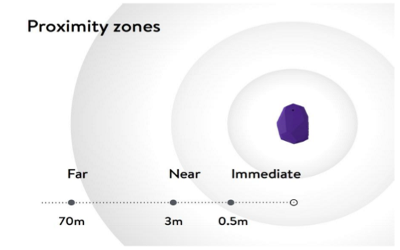
\includegraphics[width=\columnwidth]{BeaconsRange}
	\caption{Ejemplificación del rango de un beacon}
	\label{fig:beaconRange}
\end{figure}

\subsection{¿Con qué dispositivos funcionan?}

Las beacons son compatibles con todos los dispositivos que soporten Bluetooth Low Energy, pero para que las señales de los beacons sean detectadas por tu dispositivo, se ha de tener activado el Bluetooth. 


En dispositivos con IOS7 \cite{URL::IOS7} o superior, el dispositivo puede estar constantemente buscando dispositivos BLE y despertar a las aplicaciones implicadas cuando entran en el rango de los beacons, incluso estando cerradas las aplicaciones.


En dispositivos Android \cite{URL::Android} el sistema operativo no está preparado para escanear dispositivos BLE, por lo que son las aplicaciones las que se tienen que encargar de escanear las proximidades buscando beacons, esto supone que las aplicaciones tienen que estar funcionando, despiertas (aunque sea en segundo plano).

Por último en dispositivos Windows Phone \cite{URL:WindowsPhone} o Blackberry \cite{URL:Blackberry} existen diferentes niveles de compatibilidad pero en los que soportan BLE, en funcionamiento es similar al de los dispositivos Android. 

\subsection{¿Qué ventajas y desventajas tienen con respecto a otras tecnologías?}

A la hora de hablar de los beacons existen una serie de ventajas pero también podemos encontrar algunas desventajas que iremos detallando a continuación. 


Las principales ventajas que se distinguen a la hora de hablar de las beacons son las siguientes: 

\begin{itemize}
\item A diferencia de la tecnología GPS, la activación del bluetooth consume mucho menos batería. 
\item Es una tecnología que puede ser dependiente de la red de datos. 
\item A diferencia de la tecnología GPS, sigue funcionando con gran precisión en el interior de los edificios.
\end{itemize}

En cuanto a las desventajes que nos podemos encontrar destacamos:

\begin{itemize}
\item Dependen de aplicaciones instaladas en el dispositivo móvil para funcionar. 
\item Es necesario tener el bluetooth activado, lo que consume batería en el tiempo. 
\item Su utilidad depdende de la voluntad de terceros de utilizar estos dispositivos, configurarlos y distribuir las aplicaciones.
\end{itemize}

\subsection{¿Qué usos se le ha dado a esta tecnología hasta ahora?}

Por ahora esta tecnología se ha utilizado en ambiente muy diversos y con distintas funcionalidades. De los más conocidos podríamos destacar los siguientes: 

\vspace{5mm}

\textsl{\textbf{{Clevedon School (K-12)}}}

\vspace{2mm}

Este ejemplo es bastante significativo ya que se aplicó en el mismo entorno en el que queremos trabajar, una institución de enseñanza universitaria. Después de desplegar cerca de 1200 iPads  la universidad de Clevedon utilizó esta tecnología junto con su aplicación universitaria ya existente. 

\begin{figure}[H]
	\centering
	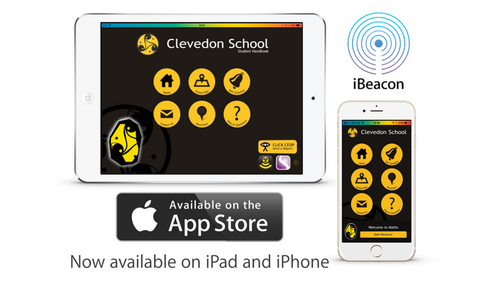
\includegraphics[width=\columnwidth]{ClevedonApp}
	\caption{La aplicación de Clevedon School}
	\label{fig:beaconRange}
\end{figure}


Han sido capaces de crear una manera fácil para que los profesores puedan añadir recursos que se envian automáticamente a los alumnos transitando diferentes zonas en diferentes horarios.Para realizar este trabajo de manera eficiente fue necesario la creación de una Interface para la gestión de los recursos en las diferentes Beacons.


Esta interfaz junto con la aplicación móvil es capaz de: 

\begin{itemize}
\item Programar los recursos para distribuirse a una hora del día especificada. 
\item Programar el material para ser distribuido en un momento determinado durante una clase o evento. 
\item Poner los recursos a disposición de los alumos que se encuentren en una localización específica.
\end{itemize}

Utilizando estos tres recursos, la aplicación, la interfaz y los beacons han sido capaces de crear un entorno interactivo y eficiente motivando tanto a profesores como estudiantes. 

\vspace{5mm}

\textsl{\textbf{{Cleveland Cavaliers Stadium y Levi's Stadium}}}

\vspace{2mm}

Dos de los ejemplos más conocidos han sido los despliegues que se han realizado en estos dos estadios. 

\begin{figure}[H]
	\centering
	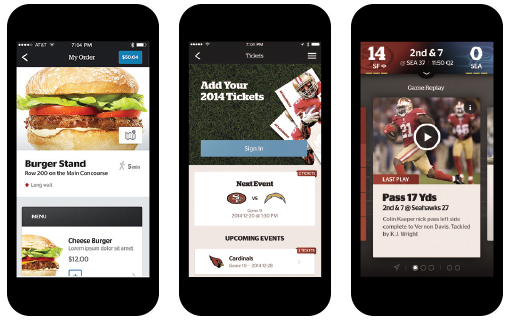
\includegraphics[width=\columnwidth]{LevisStadium}
	\caption{La aplicación de Levi's Stadium}
	\label{fig:levisStadium}
\end{figure}

Por un lado tenemos el despliegue del estadio de Levi's , cuya intención ha sido la de ayudar a sus fans a navegar por el estadio dadas sus dimensiones.En este caso los beacons (de la comañía Aruba Networks) se utilizan en conjunto con puntos de acceso y repetidores situados por toda la infraestructura de manera que queda el estadio cubierto. Con la aplicación los fans también son capaces de ver repeticiones de las jugadas y pedir comida directamente desde sus dispositivos móviles.


Un punto importante de este  despliegue ha sido la monitorización continua del funcionamiento de los beacons, incluyendo si estan en funcionamiento o necesitan bateria nueva. Los beacons son también más económicos que los puntos de acceso WiFi, lo cual les ha beneficiado.

En el caso del estadio de Cleveland, los beacons se encargan de proveer al usuario de información personalizada dependiendo del lugar y la hora. En algunos casos videos, ofertas promocionales y contenido adicional.

\vspace{5mm}

\textsl{\textbf{{Orlando Int'l Airport}}}

\vspace{2mm}

Otro despliegue exitoso de esta tecnología ha sido en el Aeropuerto Internacional de Orlando , donde mediante el uso de los beacons y de una aplicación móvil propia han sido capaces de proporcionar una serie de funcionalidades de vital importancia en una infraestructura como el aeropuerto: 

\begin{itemize}
\item Navegación paso por paso a través de cerca de 1000 establecimientos o servicios dentro del aeropuerto. 
\item Actualizaciones inmediatas de la información de los vuelos. 
\item Intrucciones a puntos de interés criticos como puntos de recogida de equipaje, puertas de embarque o puestos de información.
\end{itemize}

\begin{figure}[H]
	\centering
	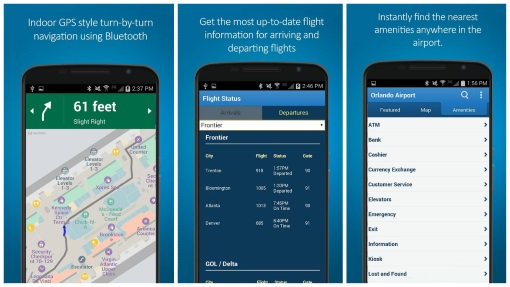
\includegraphics[width=\columnwidth]{orlandoAirport}
	\caption{La aplicación del Aeropuerto Internacional de Orlando}
	\label{fig:orlandoAirport}
\end{figure}

El siguiente punto sería ampliar la opción a los establecimientos de ofrecer anuncios o promociones, opción que mantienen abierta y no se descarta en un futuro.

%Articulos sacados de: \cite{URL::Ariculo} http://www.securedgenetworks.com/blog/3-brilliant-examples-of-how-beacon-technology-is-transforming-mobility


\section{CouchBase Server}

Couchbase Server es una base de datos NoSQL con una arquitectura distribuida orientada al rendimiento, escalabilidad y disponibilidad. Da la oportunidad a los desarrolladores a construir aplicaciones de manera sencialla y más rápida combinando la flexibilidad del JSON y la tecnología NoSQL.

\subsection{¿Por qué utilizar Couchbase Server?}

Hemos decidido utilizar esta tecnología por su flexibilidad y potencia para almacenar documentos fácilmente. Además es muy sencillo integrarla con la tecnología móvil mediante el uso de una base de datos reducida dentro del dispositivo móvil y sincronizándola con la base de datos principal del servidor mediante una puerta de sincronización.

\begin{figure}[H]
	\centering
	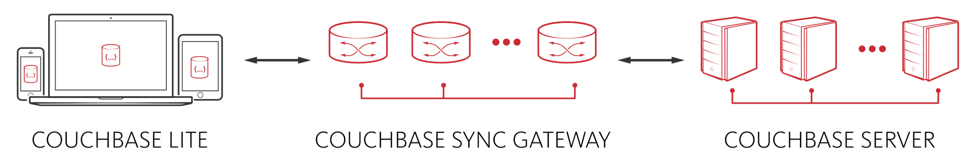
\includegraphics[width=\columnwidth]{couchbaseexplanation}
	\caption{Sincronización de CouchBase Server con CouchBase Lite mediante Sync Gateway}
	\label{fig:couchbaseexplanation}
\end{figure}

En este caso se ha configurado el servidor en un ordenador portátil haciendo uso de las indicaciones de la página web del producto. Se procederá a desglosar brevemente los pasos seguidos a la hora de configurar el servidor.


\subsection{Configuración de la arquitectura}

Para configurar el servidor se han seguido los siguientes pasos: 


\begin{itemize}
\item Descargar la versión Community del producto desde la página web siguiendo el enlace: http://www.couchbase.com/nosql-databases/downloads . 
\item Seguir los pasos de la página de desarrolladores para la intallación y configuración: http://developer.couchbase.com/documentation/server/4.5/getting-started/installing.html y 
%http://developer.couchbase.com/documentation/server/4.5/install/init-setup.html#topic12527 . 
\item Una vez configurado CouchBase Server procedemos a descargar Sync Gateway que será el servicio que se encarge de sincronizar el contenido del nuestra aplicación al servidor, para ello lo descargaremos de la página al igual que el servidor siguiendo el link: http://www.couchbase.com/nosql-databases/downloads .
\item Para vincular el servidor con Sync Gateway es necesario hacer uso de un fichero de configuración con el que lanzaremos el servicio Sync Gateway.
\item Una vez configurado Sync Gateway, ya tenemos el canal de configuración entre el servidor y la aplicación, para utilizar la base de datos móvil seguiremos los pasos desglosados en: http://developer.couchbase.com/documentation/mobile/1.2/develop/training/build-first-android-app/index.html .
\end{itemize}


En este caso, se ha tenido que conectar el dispositivo al ordenador, tanto el ordenador como el dispositivo móvil han de estar en la misma red y hemos utilizado la dirección IP de la máquina para realizar las peticiones del móvil al servidor (alojado en el portátil) al utilizar la API. De esta manera se ha comprobado el funcionamiento del servidor, del servicio de sincronización y de la base de datos versión lite en el dispositivo móvil.


\section{La librería AltBeacon}


\subsection{¿Qué es AltBeacon?}

Se puede definir AltBeacon como una especificación que: 

\begin{itemize}
\item Define el formato del mensaje publicitario que los beacons transmiten a través de BLE (Bluetooth Low Energy).
\item Intenta crear un mercado abierto y competitivo para implementaciones usando proximidad con los beacons.
\item Puede ser utilizada por todos gratuitamente, sin cuotas ni compromisos.
\item No favorece a ningún proveedor sobre otro. Las limitaciones vienen determinadas por los estándares técnicos del proveedor.
\end{itemize}

A continuación se profundizará en el funcionamiento y configuración de la librería AltBeacon, librería que cumple con la especificación AltBeacon y que se ha utilizado para trabajar en Android.

\subsection{Configuración}

Para trabajar con esta librería en Android Studio solo hemos tenido que importarla mediante el uso de Gradle a nuestro proyecto como se explica en : 

https://altbeacon.github.io/android-beacon-library/configure.html

También es posible descargarla desde la página oficial, donde además podremos econtrar diferentes versiones de la misma, para ello podemos hacer uso del siguiente enlace y seleccionar la versión deseada: 

https://altbeacon.github.io/android-beacon-library/download.html

\subsection{Funcionamiento}

Prácticamente la funcionalidad de esta librería se centra en dos elementos principales: 

\begin{itemize}
\item \textit{''Monitoring''} que sería algo así como supervisar, saber que beacons se encuentran en una región o si ha entrado o salido un beacon de una región.
\item \textit{''Ranging''} que hace referencia a rastrear, permitiendo saber a que distancia se encuentran los beacons en todo momento dentro de una región.
\end{itemize}

Utilizando estas dos funcionalidades la aplicación es capaz de controlar, monitoreando y rastreando los distintos beacons en una determinada región. En la página web de la libraría se pueden encontrar ejemplos básicos de como se realizan estas dos funciones en la sección \textit{''Samples''}, además en la sección \textit{''Documentación''} se pueden encontrar también algunos artículos, que pueden resultar interesantes dependiendo del tipo de aplicación que estes desarrollando.





%\begin{frame}
	\frametitle{La aplicación \BulletPoint{}}
	\begin{columns}
		\begin{column}{0.6\textwidth}
			\block{Localización de transporte público, horarios e información de la parada}
			\begin{itemize}
				\item Objetivo.
				\item Despliegue.
				\item Funcionamiento.
				\item Dificultades.
				\item Ampliación.
			\end{itemize}
			\endblock{}
		\end{column}
		\begin{column}{0.4\textwidth}
			\vfill 
			\begin{center}
				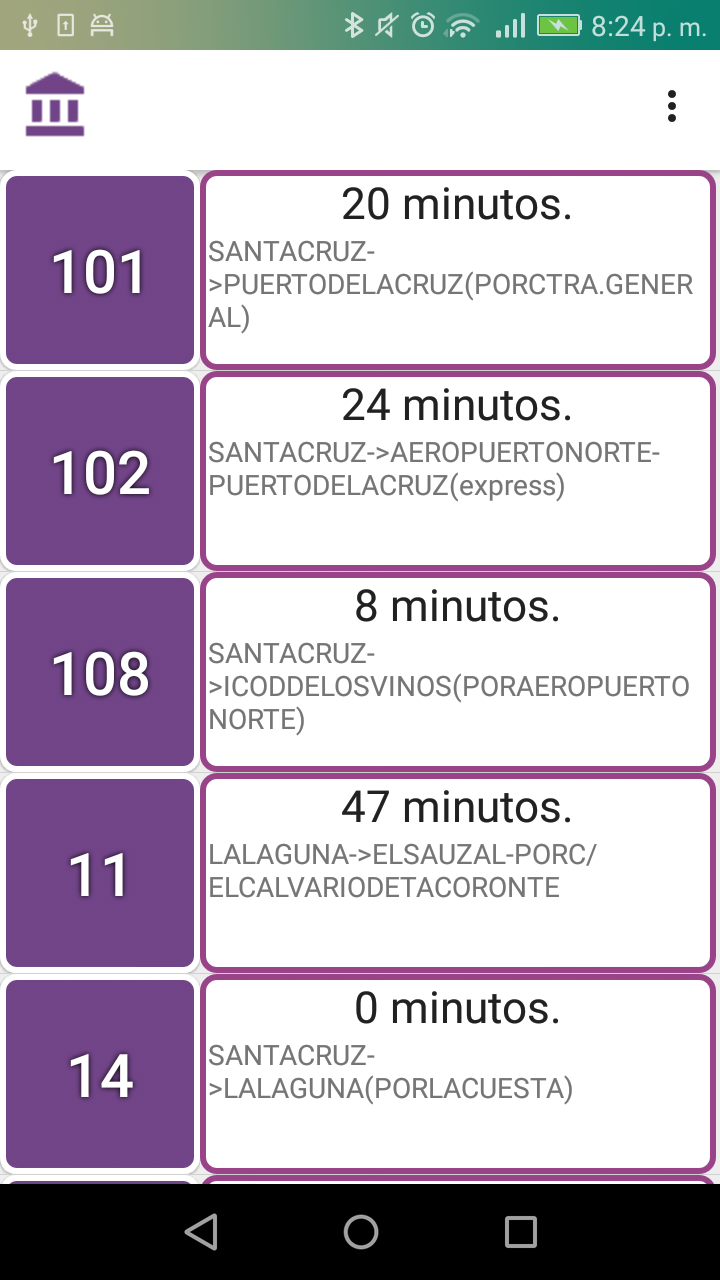
\includegraphics[width=0.8\linewidth]{Images/App/Autobuses}
			\end{center}
		\end{column}
	\end{columns}
\end{frame}

%--------------------------------------------------------------------

\begin{frame}
	\frametitle{Asociación de MAC a identificador de parada}
	\lstinputlisting{Code/BeaconBusStop.java}
\end{frame}

%--------------------------------------------------------------------

\begin{frame}
	\frametitle{Petición API TITSA}
	\lstinputlisting{Code/HttpClientTitsaJsoup.java}
\end{frame}

%--------------------------------------------------------------------

\begin{frame}
	\frametitle{La aplicación \BulletPoint{}}
	\begin{columns}
		\begin{column}{0.6\textwidth}
			\block{Gestión de eventos e información}
			\begin{itemize}
				\item Objetivo.
				\item Despliegue.
				\item Funcionamiento.
				\item Dificultades.
				\item Ampliación.
			\end{itemize}
			\endblock{}
		\end{column}
		\begin{column}{0.4\textwidth}
			\vfill 
			\begin{center}
				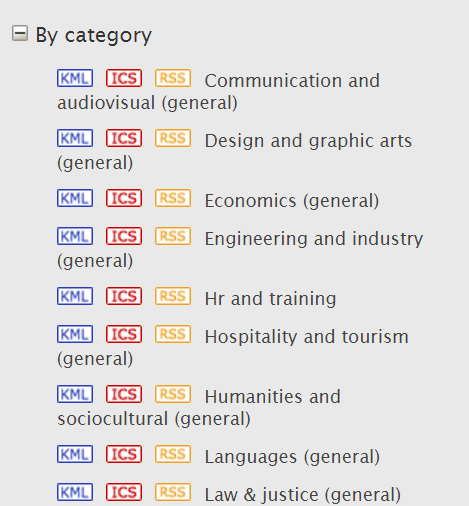
\includegraphics[width=0.7\linewidth]{Images/eventsRss}
			\end{center}
		\end{column}
	\end{columns}
\end{frame}

%--------------------------------------------------------------------

\begin{frame}
	\frametitle{Asociación de MAC a enlace RSS}
	\lstinputlisting{Code/RssBeaconInfo.java}
\end{frame}

%--------------------------------------------------------------------

\begin{frame}
	\frametitle{La aplicación \BulletPoint{}}
		\block{Control de asistencia}
		\begin{itemize}
			\item Objetivo.
			\item Despliegue.
			\item Funcionamiento.
			\item Dificultades.
			\item Ampliación.
		\end{itemize}
		\endblock{}
\end{frame}

%--------------------------------------------------------------------

\begin{frame}
	\frametitle{Preferencias de usuario}
	\lstinputlisting{Code/preferences.xml}
\end{frame}

%--------------------------------------------------------------------

\begin{frame}
	\frametitle{Comprobando la localización en el área}
	\lstinputlisting{Code/scanAtt.java}
\end{frame}

%--------------------------------------------------------------------

\begin{frame}
	\frametitle{La aplicación \BulletPoint{}}
		\block{Guía a través del campus de la universidad}
		\begin{itemize}
			\item Objetivo.
			\item Despliegue.
			\item Funcionamiento.
			\item Dificultades.
			\item Ampliación.
		\end{itemize}
		\endblock{}
\end{frame}

%--------------------------------------------------------------------

\begin{frame}
	\frametitle{Mostrar la posición del usuario en la imagen}
	\lstinputlisting{Code/threeMainFunctionTrilaterate.java}
\end{frame}

\begin{frame}
	\frametitle{La aplicación \BulletPoint{}}
	\begin{columns}
		\begin{column}{0.6\textwidth}
			\block{Acceso al parking}
			\begin{itemize}
				\item Objetivo.
				\item Despliegue.
				\item Funcionamiento.
				\item Dificultades.
				\item Ampliación.
			\end{itemize}
			\endblock{}
		\end{column}
		\begin{column}{0.4\textwidth}
			\vfill 
			\begin{center}
				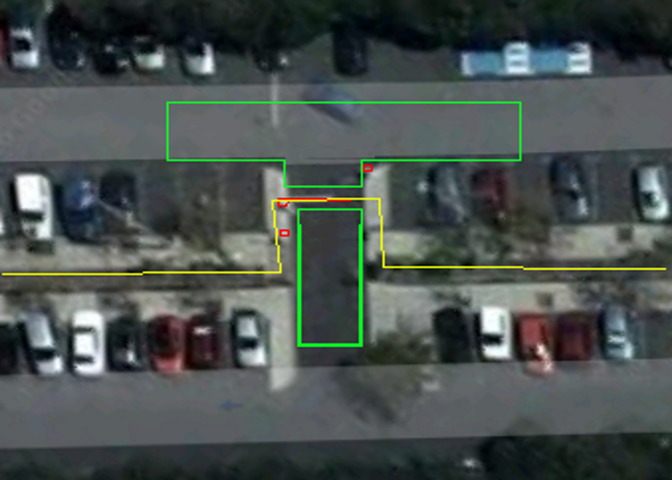
\includegraphics[width=0.9\linewidth]{Images/parking}
			\end{center}
		\end{column}
	\end{columns}
\end{frame}

%--------------------------------------------------------------------

\begin{frame}
	\frametitle{La aplicación \BulletPoint{}}
		Vídeo demostrativo de la aplicación \BulletPoint{}
\end{frame}
%\begin{frame}
  \frametitle{Despliegue}
  \block{Repositorio de la aplicación}
    \begin{itemize}
		\item La aplicación ha sido almacenada en el repositorio GitHub como parte del PATFL.
    \item Se encuentra en GitHub: https://github.com/ccetsii/BulletPoint 
    \end{itemize}
  \endblock{}
\end{frame}
%\include{Cap6_todo}
%\include{Cap7_SummaryClonclusions}
%\include{Cap8_Presupuesto}

%\newpage{\pagestyle{empty}}
%\thispagestyle{empty}

%\chapter{Presupuesto}
%\label{chapter:Presupuesto}

%\input{cap7.tex}

%%%%%%%%%%%%%%%%%%%%%%%%%%%%%%%%%%%%%%%%%%%%%%%%%%%%%%%%%%%%%%%%%%%%%%%%%%%%%%%

%%%%%%%%%%%%%%%%%%%%%%%%%%%%%%%%%%%%%%%%%%%%%%%%%%%%%%%%%%%%%%%%%%%%%%%%%%%%%%%
%\newpage{\pagestyle{empty}}
%\thispagestyle{empty}
%\begin{appendix}
%
%\chapter{Título del Apéndice 1}
%\label{appendix:1}
%\input{apendice1.tex}
%
%\chapter{Título del Apéndice 2}
%\label{appendix:2}
%\input{apendice2.tex}
%
%\end{appendix}
%%%%%%%%%%%%%%%%%%%%%%%%%%%%%%%%%%%%%%%%%%%%%%%%%%%%%%%%%%%%%%%%%%%%%%%%%%%%%%%
\addcontentsline{toc}{chapter}{Bibliografía}
\bibliographystyle{plain}
\renewcommand{\bibname}{Bibliografía}   %  Para que no aparezca Índice de figuras
\bibliography{bibliografia}

%%%%%%%%%%%%%%%%%%%%%%%%%%%%%%%%%%%%%%%%%%%%%%%%%%%%%%%%%%%%%%%%%%%%%%%%%%%%%%%

\end{document}
